\begin{exercise}
\begin{figure}[H]
\centering

\includegraphics[width=\textwidth]{hw8-2025061023.png}
% \caption{}
\label{}
\end{figure}
\begin{figure}[H]
\centering
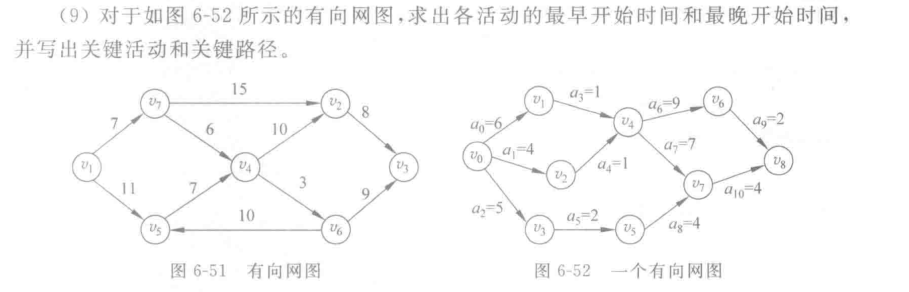
\includegraphics[width=\textwidth]{1-hw8-2025061023.png}
% \caption{}
\label{}
\end{figure}
\end{exercise}
\begin{figure}[H]
\centering
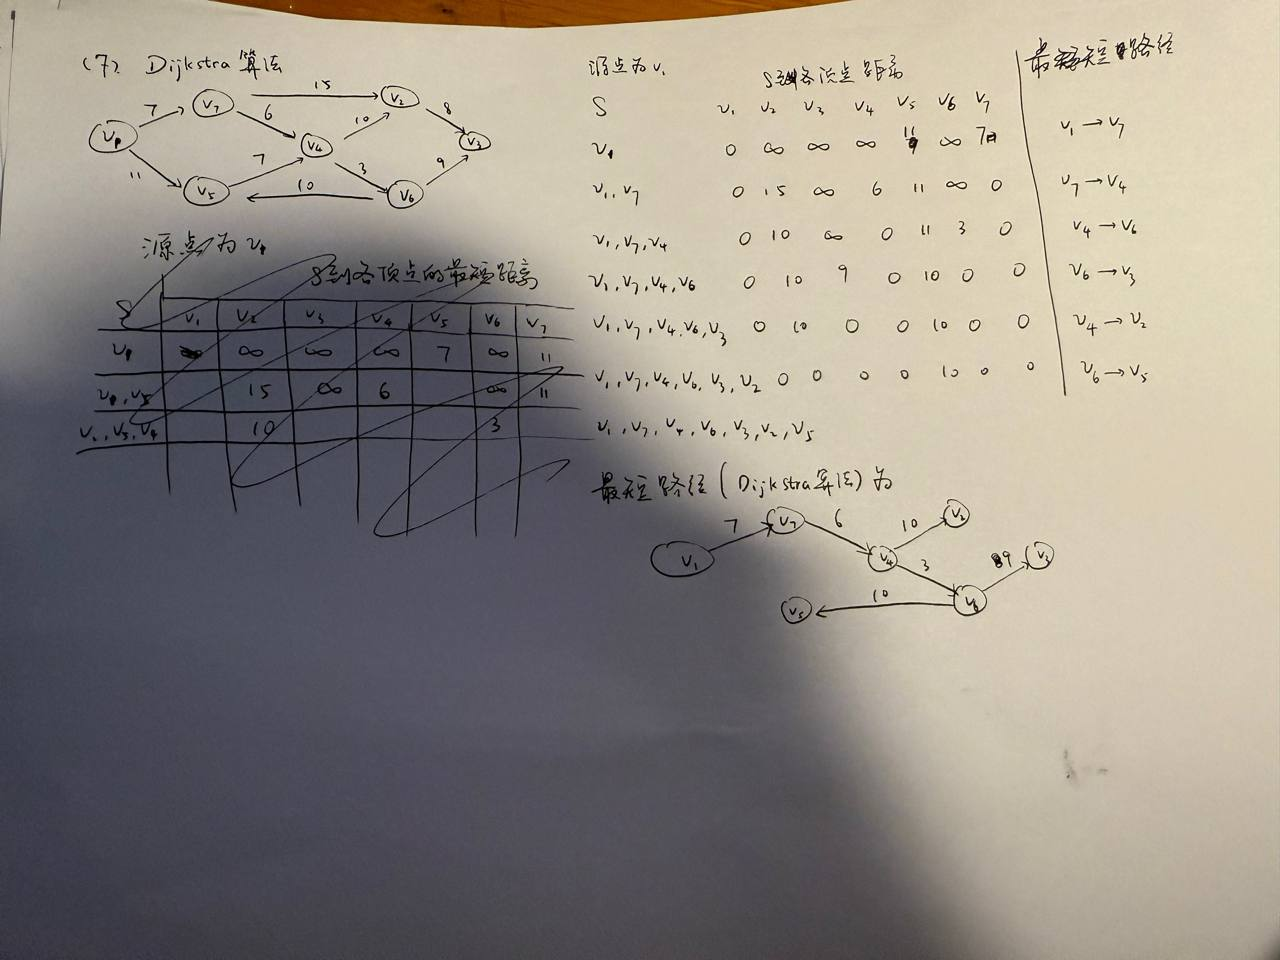
\includegraphics[width=\textwidth]{hw8-2025061623.png}
% \caption{}
\label{}
\end{figure}

\begin{figure}[H]
\centering
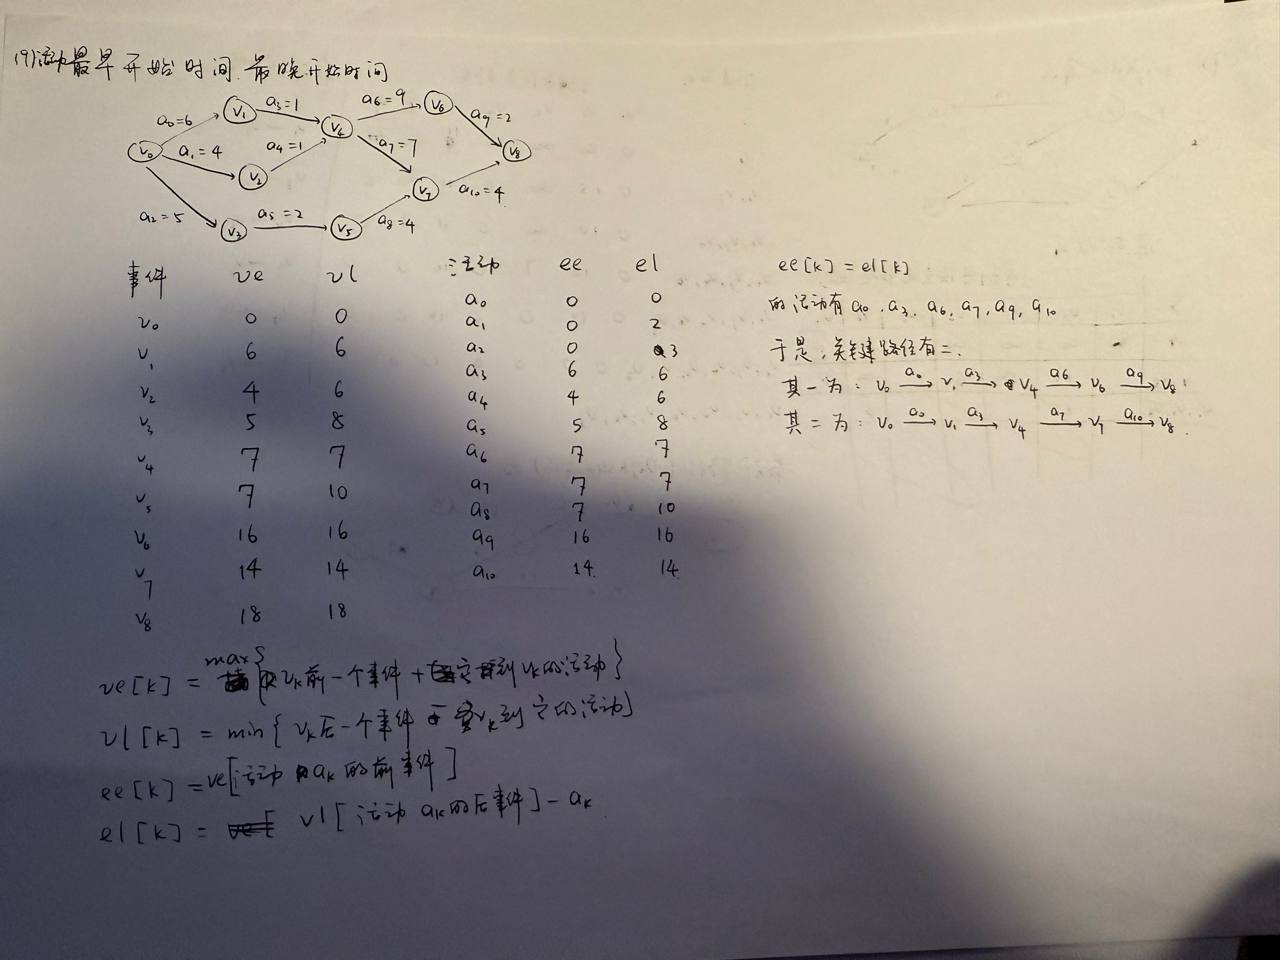
\includegraphics[width=\textwidth]{hw8-2025061721.png}
% \caption{}
\label{}
\end{figure}

\begin{exercise}
\begin{figure}[H]
\centering

\includegraphics[width=\textwidth]{3-hw8-2025061023.png}
% \caption{}
\label{}
\end{figure}
\begin{figure}[H]
\centering

\includegraphics[width=\textwidth]{4-hw8-2025061023.png}
% \caption{}
\label{}
\end{figure}
\end{exercise}
(5)

\begin{lstlisting}
Algorithm DFS_SpanningTree(Graph G):
    Input:Graph G=(V,E)
	Output:A list of edges representing the DFS spanning tree
	
	Initialize visited[v] = false for allv in V
	Initialize dfs_tree_edges = []
	
	For each vertex vin V:
	    If not visited[v]:    
	        DFS_visit(v, visited, dfs_tree_edges)
	        
	Return dfs_tree_edges
	
Algorithm DFS_Visit(u, visited, dfs_tree_edges):
	visited[u] = true
	For each neighbor w of u:
	    If not visited[w]:
	        Add edge (u, w) to dfs_tree_edges
	        DFS_Visit(w, visited, dfs_tree_edges)
\end{lstlisting}
(7)

算法步骤:

\begin{enumerate}
	\item 初始化一个数组 status,所有元素设为 0 (未访问)。
	\item 遍历图中的每一个顶点 $v$:
\end{enumerate}

\begin{itemize}
	\item 如果 status[v]为 0 (未访问):
	\item 调用 HasCycleDFS(v,status,adj\_matrix)。
	\item 如果 HasCycleDFS 返回 true,则表示存在回路,立即返回 true。
\end{itemize}

\begin{enumerate}
	\item 如果遍历完所有顶点都没有发现回路,则返回 false。
\end{enumerate}

HasCycleDFS(u,status,adj\_matrix)函数:

\begin{enumerate}
	\item 将 status[u]设为 1 (正在访问)。
	\item 对于顶点 $u$ 的每一个邻接顶点 $w$(即 adj\_matrix $[u][w]==1$ ):
\end{enumerate}

\begin{itemize}
	\item 如果 status[w]为 1 (正在访问):
	\item 返回 true(发现回路)。
	\item 如果 status[w]为 0 (未访问):
	\item 如果递归调用 HasCycleDFS(w,status,adj\_matrix)返回 true,则返回 true。
\end{itemize}

\begin{enumerate}
	\item 将 status[u]设为 2 (已访问完成)。
	\item 返回 false(以 $u$ 为起点的 DFS 路径未发现回路)。
\end{enumerate}


(8)

DFS:

\begin{enumerate}
	\item 初始化一个布尔数组visited,所有元素设为false。
	\item 调用 DFS\_PathExists (v\_i,v\_j,visited,adj\_list)。
\end{enumerate}

DFS\_PathExists(u,target\_v,visited, adj\_list) 函数:

\begin{itemize}
	\item 如果u等于target\_v,返回true(找到路径)。
	\item 将visited[u]设为true。
	\item 对于顶点u的每一个邻接顶点w:
	\begin{itemize}
		\item 如果w未被访问过:
		\item 如果递归调用 DFS\_PathExists(w,target\_v,visited,adj\_list)返回true,则返回true。
	\end{itemize}
	\item 返回false(从u出发无法到达target\_v)。
\end{itemize}

BFS:

\begin{enumerate}
	\item 初始化一个布尔数组visited,所有元素设为false。
	\item 创建一个队列Q并将v\_i加入队列。
	\item 将visited[v\_i]设为true。
	\item 当队列不为空时:
	\begin{itemize}
		\item 从队列中取出一个顶点u。
		\item 如果u等于v\_j,返回true(找到路径)。
		\item 对于顶点u的每一个邻接顶点w:
		\begin{itemize}
			\item 如果w未被访问过:
			\begin{itemize}
				\item 将visited[w]设为true。
				\item 将w加入队列。
			\end{itemize}
		\end{itemize}
	\end{itemize}
	\item 如果队列为空且未找到v\_j,则返回false。
\end{enumerate}
